\documentclass{beamer}
\usepackage[english,french]{layout}
\usepackage[utf8]{inputenc}
\usepackage[english]{babel}
\usepackage[T1]{fontenc}
\usepackage{lmodern}
\usepackage{textcomp}
\usepackage{amsmath, soul, color, multicol, type1cm, verbatim, latexsym, dsfont, float, listings,alltt}
\usepackage[official]{eurosym}
\usepackage{beamerthemesplit}
\usetheme{Frankfurt}
\usefonttheme{professionalfonts}
\setbeamercovered{transparent}
%NeSI Colors <-------------------------------------------------------------------------------------
\usecolortheme{lily}
\usecolortheme[RGB={47, 68, 71}]{structure} 
\definecolor{nesidark}{HTML}{2F4447}
\definecolor{nesilight}{HTML}{CED9DF}
\definecolor{nesigrey}{gray}{0.7}
\definecolor{nesilightgrey}{gray}{0.98}
\definecolor{nesidarkgrey}{gray}{0.3}
\definecolor{nesiblue}{HTML}{2B9FC2}
\setbeamercolor{block title}{fg=black,bg=nesigrey}
\setbeamercolor{block body}{bg=nesilightgrey,fg=nesidarkgrey}
\setbeamercolor{block body alerted}{bg=white,fg=black}
\setbeamercolor{alerted text}{bg=white,fg=black}
%NeSI Title <---------------------------------------------------------------------------------------
\setbeamerfont{title}{size=\huge}
\frenchspacing
\hyphenation{NeSI}
%NeSI Template parameters <-------------------------------------------------------------------------
\setbeamertemplate{blocks}[default]
\useinnertheme{circles}
\setbeamertemplate{title page}[default][center,rounded=false,shadow=false]
\newcommand\BackgroundPicture[1]{%
\setbeamertemplate{background}{%
\parbox[c][\paperheight]{\paperwidth}{%
\vfill \hfill \includegraphics[height=0.9\paperheight]{#1}
\hfill \vfill
}}}

%Content Starts Here <-------------------------------------------------------------------------------
\title{Enabling High--Throughput Research on HPC Systems}
%\subtitle{Computational Science team}
\author{Dr Fran{\c c}ois Bissey \\ (francois.bissey@canterbury.ac.nz)}
\date{}

\begin{document}

{
\setbeamertemplate{background canvas}{
\includegraphics[height=0.99\paperheight]{NeSI_img/Slide00.png}} 
\begin{frame}[plain]
\vspace{1cm}
\titlepage
\end{frame}
}


\begin{frame}
\frametitle{Outline}
   \tableofcontents
\end{frame}


\section{Introduction}

\frame[t]
{
\frametitle{Introduction}
\begin{block}{Two types of fundamental workflow for HPC}
\begin{itemize}
 \item Large distributed memory (MPI) jobs
 \item High-throughput jobs
\end{itemize}
\end{block}

\begin{block}{High-throughput jobs covers}
\begin{itemize}
 \item Monte-Carlo simulations
 \item Parameter space sweeps
 \item Processing of large data sets
\end{itemize}
It is characterised by doing a task over and over again with a different input.
\end{block}
}

\section{The Problem}

\frame[t]
{
\frametitle{The problem}
\begin{block}{MPI machines}
Machine like the Power7 cluster at BlueFern and Fitzroy at NIWA are geared towards distributed memory jobs (MPI).
\end{block}

\begin{block}{High-throughput job}
Running high-throughput jobs efficiently on these systems requires a little bit of thinking ahead and care.
We will "steal" the MPI workflow to achieve this. Machines like Pan in Auckland are geared more towards high-throughput and medium size MPI jobs but applying the techniques presented here could be beneficial on it as well.
\end{block}
}

\subsection{Ehsan's Simulations}
\frame[t]{
\frametitle{Ehsan's Simulations}
Ehsan is a PhD student in computer science. His problem is simulating wireless networks to improve the efficiency of the communication in mobile devices.

\begin{itemize}
\item first submission to the cluster was 40,000 simulations
\item done 4 at a time
\item first reaction: increase the number of simulations he can run (after all they are not big MPI jobs)
\item Bad idea: the simulations were spread all over the cluster blocking big MPI jobs
\item developed a custom solution to contain him to a set of nodes
\item we later found out that it was equivalent to using MPMD
\end{itemize}
We now identify high-throughput projects quickly and offer them better solutions as soon as possible.
}

\section{Solutions}

\subsection{presentation}
\frame[t]{
\frametitle{Solutions}
\begin{block}{Presentation}
There are two main ways of packaging serial jobs to pass them as MPI distributed memory job, we'll look at them through the work of two researchers.
\begin{enumerate}
 \item MPMD (Multiple Program Multiple Data): Nick's network
 \item Batcher: Jing Wang DNA matching work
\end{enumerate}
\end{block}
}

\subsection{Nick's networks}
\frame[t]{
\frametitle{Nick's Networks}
\begin{itemize}
\item Nick Baker is a PhD student in biological sciences with a background in mathematics. He studies ecological networks (complex food chains).

\item His work focuses on analysing networks to find "keystone" species that are essential to the network. The work is what we call embarrassingly parallel, he has to go through a high number of networks and perform his analyses on each and every one of them.

\item I spotted him on the cluster running four jobs at a time out of close to a hundred. There was definitely room for improvement. He became a test subject for MPMD
\end{itemize}
}
\frame[t]{
\frametitle{MPMD: Multiple Program Multiple Data}
\begin{multicols}{2}
\begin{figure}
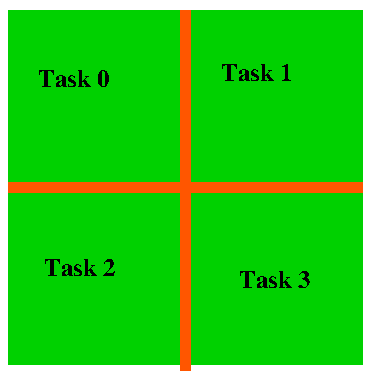
\includegraphics[scale=0.5]{smpd_task.pdf}
\end{figure}
\begin{center}
SMPD: Instances of a program process the data distributed amongst them.
\end{center}
\begin{figure}
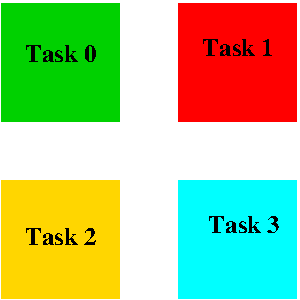
\includegraphics[scale=0.5]{mpmd_task.pdf} 
\end{figure}
\begin{center}
MPMD: Programs, not necessarily identical, process distinct data.
\end{center}
\end{multicols}
}

\begin{frame}[fragile]
\frametitle{MPMD jobs at BlueFern (and Fitzroy)}
At BlueFern and Fitzroy, such jobs can be launched with the following
\begin{small}
\begin{verbatim}
poe -procs N -pgmmodel mpmd -cmdfile cmdfile.txt
\end{verbatim}
\end{small}
Where \textit{cmdfile.txt} is a list of commands to be executed
\begin{small}
\begin{verbatim}
program1 data1
program2 data2
...
programN dataN
\end{verbatim}
\end{small}
Note that the number of commands matches the number of cores requested. Now, Nick usually processes 32 networks per job instead of one.
\end{frame}

\subsection{Jing Wang, DNA matching with batcher}
\frame[t]{
\frametitle{Jing Wang, DNA matching with batcher}
\begin{itemize}
\item Jing Wang is a researcher at ESR and came to us for several NeSI research projects
\item The problem is to compare strands of DNA against a database to match sequences of genes
\item The task can be further broken down by splitting the strands in sections and searching for match in these. 
\item Searching for sequences in one long DNA strand can take a long time. Doing it on a section is much quicker but now you have to do it on potentially thousands of sections. This has become a high-throughput task.
\end{itemize}
}

\frame[t]{
\frametitle{Batcher: Master and Worker}
A batcher program uses a different MPI mode: the ability for one program to be a master that spawns workers to do various jobs on demand.

Like MPMD, the batcher program will take a list of tasks. Unlike MPMD, however, batcher does not start all tasks at once. If you give batcher more tasks than you have cores, it will fill the cores given. When one task finishes, it will start the next one in the list until all tasks are completed.

Instead of building packets to match the number of cores requested (MPMD) you can package in units that make sense.
}

\begin{frame}[fragile]
\frametitle{Batcher jobs at BlueFern}
At BlueFern such jobs can be launched with the following
\begin{small}
\begin{verbatim}
poe batcher cmdfile.txt
\end{verbatim}
\end{small}
Where \textit{cmdfile.txt} is a list of commands to be executed
\begin{small}
\begin{verbatim}
program1 data1 >> out1.log
program2 data2 >> out2.log
...
programN dataN >> outN.log 
\end{verbatim}
\end{small}
\end{frame}

\section{Pros and Cons}
\frame[t]{
\frametitle{Pros and Cons}
\begin{multicols}{2}
\begin{block}{Batcher}
Pros:
\begin{itemize}
\item Can group any number of tasks
\item tasks that complete quickly will be replaced by new tasks while the longer ones finish
\end{itemize}
Cons:
\begin{itemize}
\item one core is used by batcher and not available to do tasks
\end{itemize}
\end{block}
\begin{block}{MPMD}
Pros:
\begin{itemize}
\item all cores are used
\end{itemize}
Cons: 
\begin{itemize}
\item if some tasks are much longer than others some cores will be idle
\item number of tasks must be equal to number of cores
\end{itemize}
\end{block}
\end{multicols}
}

\section{Conclusions}
\frame[t]{
\frametitle{Conclusions}
\begin{itemize}
\item Lots of serial jobs are not a good thing on a machine tuned for MPI jobs
\item We solve this by packing the serial jobs in a way that make look like MPI jobs
\item It increases your throughput at BlueFern and Fitzroy
\item It makes the life of your cluster administrator easier
\item MPMD is best suited for tasks of equal length (lattice QCD, Monte-Carlo)
\item batcher is best suited for the rest
\item Jobs can also be packaged on the Pan cluster in Auckland but the MPMD submission would be different.
\end{itemize}
}
{
\setbeamertemplate{background canvas}{
\includegraphics[height=0.99\paperheight]{NeSI_img/Slide00.png}} 
\begin{frame}[plain]
\begin{center}
{\Huge Questions \& Answers}
\end{center}
\end{frame}
}


\end{document} 
